\documentclass[14pt]{extreport}

\usepackage[utf8]{inputenc}
\usepackage[T2A]{fontenc}
\usepackage[english,ukrainian]{babel}
\usepackage{tempora}

\usepackage{float}
\usepackage{caption}
\captionsetup[table]{justification=raggedleft, singlelinecheck=false, labelsep=period}
\captionsetup[figure]{labelsep=space}
\usepackage{graphicx}
\graphicspath{ {./pictures} }
\usepackage{listings}
\lstset{breaklines=true,showstringspaces=false}
\linespread{1.5}
\setlength{\parskip}{0pt}
\usepackage{indentfirst}

\usepackage[a4paper,top=20mm,bottom=20mm,left=25mm,right=10mm]{geometry}

\usepackage{fancyhdr}
\fancypagestyle{plain}{
  \pagestyle{myheadings}
}
\pagestyle{myheadings}

\usepackage{titlesec}
\titleformat{\chapter}{\centering\bfseries\MakeUppercase}{}{1pc}{}
\titleformat{\section}{\centering\bfseries\MakeUppercase}{}{1pc}{}
\titleformat{\subsection}{\bfseries}{}{1pc}{}
\titleformat{\subsubsection}{\bfseries}{}{1pc}{}
% \titleformat{\paragraph}{\bfseries}{}{}{}

\titlespacing*{\chapter}{0pt}{10mm}{14pt}
\titlespacing*{\section}{\parindent}{14pt}{0pt}
\titlespacing*{\subsection}{\parindent}{0pt}{0pt}
\titlespacing*{\subsubsection}{\parindent}{0pt}{0pt}
\titlespacing*{\paragraph}{\parindent}{0pt}{7pt}

\usepackage{enumitem}
\setlist{nolistsep}

\usepackage{hyperref}
\def\UrlBreaks{\do\/\do-}
\makeatletter
\renewcommand{\thesection}{\@arabic\c@section}
\makeatother

\begin{document}

\setcounter{page}{2}
\tableofcontents
\newpage

\section{Короткий опис бази практики}

\subsection{Фокусні галузі}
Основними напрямками діяльності бази практики є розробка програмного забезпечення з використанням блокчейн-технологій, створення децентралізованих застосунків (dApp), надання консалтингових послуг у сфері Web3 та смарт-контрактів, а також дослідження новітніх підходів до забезпечення безпечної взаємодії користувачів у розподілених системах.

\subsection{Технічні й програмні засоби}
У роботі використовуються такі технічні та програмні засоби, як мова програмування Rust для розробки смарт-контрактів, інструменти Solana CLI, Solana SDK та Anchor Framework. Клієнтська частина розробляється на основі Wasm або Web3 бібліотек. Для контролю версій застосовуються Git та GitHub, а серед середовищ розробки використовуються VS Code та Neovim.

\subsection{Характер робіт, пов’язаних із застосуванням ІТ}
Характер робіт передбачає створення прикладного програмного забезпечення з використанням сучасних середовищ розробки та засобів командного рядка. Важливим аспектом є робота з системами контролю версій для ефективного керування кодовою базою, а також налаштування локального середовища розробки та тестування. Студенти будуть залучені до роботи з документацією, технічними специфікаціями та вимогами до програмного забезпечення, інтеграції криптографічних механізмів підпису й перевірки транзакцій, а також до формування технічної звітності та проектної документації.

\section{Завдання, отримане на базі практики}

\begin{enumerate}
	\item Ознайомитись із основами технології блокчейн та принципами її застосування.
	\item Вивчити екосистему Solana та її програмну модель для створення смарт-контрактів.
	\item Створити простий смарт-контракт (on-chain програму).
	\item Розробити клієнтську частину для взаємодії зі смарт-контрактом.
	\item Провести локальне тестування розробленої системи за допомогою тестової мережі Solana.
	\item Забезпечити базову перевірку автентичності користувачів шляхом підпису транзакцій гаманцем.
\end{enumerate}

\section{Результати виконання завдання на базі практики}

Проведено детальне вивчення теоретичних аспектів технології блокчейн. Це включало аналіз її архітектури, принципів децентралізації, методів криптографічного захисту даних та алгоритмів досягнення консенсусу між учасниками мережі. Особлива увага приділялася розумінню переваг блокчейн, таких як підвищена прозорість, незмінність даних та відсутність потреби у централізованому управлінні, а також обмежень, пов'язаних з масштабованістю та швидкістю обробки транзакцій. Досліджено приклади застосування блокчейн у різних сферах, включаючи фінансові операції, управління ланцюгами поставок та інші області, де важлива надійність та прозорість даних.

Було здійснено глибоке занурення в екосистему блокчейн-платформи Solana. Це передбачало вивчення її технічних характеристик, включаючи архітектуру, механізм консенсусу Proof of History (PoH), який забезпечує високу швидкість обробки транзакцій, та інструменти розробки, доступні для створення децентралізованих застосунків. Значну увагу було приділено програмній моделі Solana для розробки смарт-контрактів (on-chain програм). Це включало вивчення принципів організації даних у блокчейні, механізмів обробки транзакцій та взаємодії між різними смарт-контрактами. Було освоєно ключові інструменти розробки, такі як Solana Command Line Interface (CLI), Solana Software Development Kit (SDK) та фреймворк Anchor, що спрощує процес створення та розгортання смарт-контрактів.

В рамках практичної роботи було розроблено та реалізовано простий смарт-контракт, який слугує демонстрацією базових принципів роботи з платформою Solana. Цей смарт-контракт містить функції для ініціалізації змінної, її збільшення та зчитування значення. Розроблений смарт-контракт було протестовано з використанням локального середовища розробки та тестової мережі Solana для забезпечення його коректної роботи та відповідності визначеним вимогам.

Для наочної демонстрації взаємодії з розробленим смарт-контрактом було створено простий веб-додаток. Цей додаток надає користувачеві можливість переглядати поточне значення лічильника, що зберігається у блокчейні Solana, а також збільшувати це значення на одиницю за допомогою натискання на кнопку. Кожна операція збільшення лічильника вимагає підтвердження транзакції користувачем через його криптовалютний гаманець, що забезпечує прозорість та контроль над зміною даних.

\begin{figure}[H]
	\centering
	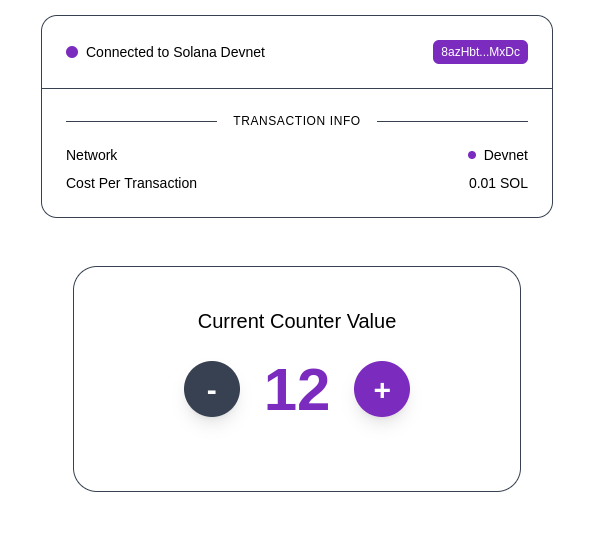
\includegraphics[scale=0.5]{1}
	\caption{Вигляд інтерфейсу}
\end{figure}

Паралельно з розробкою смарт-контракту було створено клієнтську частину застосунку. Ця частина забезпечує зручний графічний інтерфейс для взаємодії користувача зі смарт-контрактом. Клієнтська частина була розроблена з використанням технологій React для створення інтерфейсу та Web3.js для взаємодії з блокчейном. Вона забезпечує можливість відображення даних зі смарт-контракту, введення даних для виклику функцій смарт-контракту та відображення результатів. Було забезпечено інтеграцію клієнтської частини з криптовалютним гаманцем Phantom Wallet для забезпечення безпечної аутентифікації користувачів та підпису транзакцій.

Для забезпечення якості та надійності розробленої системи було проведено комплексне локальне тестування. Це передбачало налаштування локального середовища розробки, включаючи розгортання тестової мережі Solana, яка імітує роботу реальної блокчейн-мережі. Було проведено тестування смарт-контракту та клієнтської частини, включаючи перевірку функціональності, безпеки, зручності використання та продуктивності. В процесі тестування було виявлено та усунено ряд помилок та недоліків, що дозволило забезпечити стабільну та надійну роботу системи.

Для забезпечення безпеки та цілісності даних було реалізовано механізм перевірки автентичності користувачів. Цей механізм базується на використанні криптовалютного гаманця користувача для підпису кожної транзакції. Підпис транзакції приватним ключем користувача гарантує, що транзакція була ініційована саме цим користувачем і що дані не були змінені в процесі передачі. Було проведено тестування цього механізму для перевірки його надійності та стійкості до атак.

\section{Завдання стосовно дипломного проекту}

\begin{enumerate}
	\item Підготувати оглядовий розділ БКР, який включатиме теоретичні основи технології блокчейн та екосистеми Solana.
  \item Сформувати постановочний розділ БКР, де буде обґрунтовано актуальність розробки, визначено мету і завдання дослідження, а також описано предмет і об'єкт розробки.
  \item Розробити проектний розділ БКР, який детально описуватиме розроблений смарт-контракт та клієнтську частину, включаючи їхню архітектуру, функціональність та процес тестування.
\end{enumerate}

\section{Опис проведених робіт стосовно БКР}

У рамках переддипломної практики було проведено значний обсяг робіт, спрямованих на підготовку бакалаврської кваліфікаційної роботи. Зокрема, було розроблено оглядовий, постановочний та проектний розділи, які закладають теоретичний та методологічний фундамент для подальшого дослідження та розробки системи електронного голосування.

 В оглядовому розділі було здійснено комплексний аналіз існуючих наукових публікацій, літературних джерел та технологічних рішень у сфері електронного голосування.

У процесі дослідження було детально розглянуто:

\begin{itemize}
  \item основи технології блокчейн, її ключові принципи та архітектуру;
\item методи досягнення консенсусу в розподілених системах, включаючи порівняльний аналіз різних алгоритмів (PoW, PoS, PoH);
\item інноваційні підходи до організації електронного голосування, зокрема застосування блокчейн-технологій та криптографічних методів;
\item існуючі системи електронного голосування, їхні переваги та недоліки, а також аналіз можливостей та обмежень централізованих і децентралізованих рішень.
\end{itemize}

Результати проведеного аналізу дозволили сформувати чітке розуміння сучасного стану розвитку технологій електронного голосування та визначити найбільш перспективні напрями подальших досліджень.

 На основі вивчених матеріалів було сформульовано мету та завдання бакалаврської кваліфікаційної роботи.

У постановочному розділі:

\begin{itemize}
 \item обґрунтовано актуальність розробки системи електронного голосування на основі блокчейн-технології;
\item визначено мету роботи, яка полягає у створенні функціональної та надійної системи, що забезпечує прозорість, безпеку та довіру до процесу волевиявлення;
\item сформульовано конкретні завдання, необхідні для досягнення поставленої мети, включаючи розробку архітектури системи, реалізацію програмних компонентів, інтеграцію з криптовалютним гаманцем, тестування системи та підготовку технічної документації;
\item охарактеризовано об'єкт проєктування – децентралізовану систему електронного голосування, визначено вхідні дані та очікувані результати роботи системи;
\item обґрунтовано вибір технологій та методів розробки, зокрема блокчейн-платформи Solana, мови програмування Rust, бібліотеки Anchor, гаманця Phantom Wallet та фреймворку React;
\item проведено аналіз вимог до системи, включаючи функціональні та нефункціональні вимоги з точки зору організаторів голосувань та учасників.
\end{itemize}

 У розділі проектування було розроблено загальні проектні рішення:
 
 \begin{itemize}
   \item визначено основні характеристики продукту, включаючи можливості ініціювання голосувань, безпечної участі та перегляду результатів;
\item описано класи користувачів системи (організатор голосування та учасник голосування) та їхні характеристики; 
 \end{itemize}

Проведена робота над оглядовим, постановочним та проектним розділами є важливою передумовою для успішної розробки та впровадження ефективної системи електронного голосування.

\section*{Висновки}
\addcontentsline{toc}{section}{Висновки про отримані результати}

У ході практики вивчено теоретичні основи блокчейн та екосистему Solana. Розроблено простий смарт-контракт і клієнтську частину для взаємодії з ним, включаючи базову автентифікацію користувачів через криптогаманець. Проведено локальне тестування розробленої системи.

Також виконано значний обсяг робіт для бакалаврської кваліфікаційної роботи, включаючи підготовку оглядового, постановочного та проектного розділів, що закладають теоретичну та методологічну основу для дослідження системи електронного голосування на базі блокчейн-технологій.

\newpage
\section*{Список використаних джерел}
\addcontentsline{toc}{section}{Список використаних джерел}

\begin{enumerate}
\item Nakamoto, S. (2008). Bitcoin: A Peer-to-Peer Electronic Cash System. (Електронний ресурс). Посилання: \href{https://bitcoin.org/bitcoin.pdf}{https://bitcoin.org/bitcoin.pdf}
\item Solana Foundation. (n.d.). Solana Documentation. (Електронний ресурс). Посилання: \href{https://docs.solana.com/}{https://docs.solana.com/}
\item Anchor Framework. (n.d.). Anchor Book. (Електронний ресурс). Посилання: \href{https://www.anchor-lang.com/book}{https://www.anchor-lang.com/book}
\item Phantom Wallet. (n.d.). Phantom - Solana Wallet. (Електронний ресурс). Посилання: \href{https://phantom.app/}{https://phantom.app/}

\end{enumerate}

\newpage

\section*{Додаток А.\hspace{0.5em} Код програми}
\addcontentsline{toc}{section}{Додатки}
{\small
\begin{lstlisting}
use anchor_lang::prelude::*;
use anchor_lang::system_program;

declare_id!("DGmJsbjsife1p3QoueUruomvJXLaYXMwqEFgE4bV4xrg");

#[program]
mod solana_counter {
    use super::*;

    pub fn initialize(ctx: Context<Initialize>) -> Result<()> {
        let counter = &mut ctx.accounts.counter;
        counter.count = 0;
        Ok(())
    }

    pub fn increment(ctx: Context<Increment>, payment: u64) -> Result<()> {
        let counter_account_info = ctx.accounts.counter.to_account_info();
        let user = &ctx.accounts.user;

        const MINIMUM_PAYMENT: u64 = 10_000_000; // 0.01 SOL dalam lamports
        require!(payment >= MINIMUM_PAYMENT, ErrorCode::InsufficientPayment);

        let cpi_context = CpiContext::new(
            ctx.accounts.system_program.to_account_info(),
            system_program::Transfer {
                from: user.to_account_info(),
                to: counter_account_info,
            },
        );
        system_program::transfer(cpi_context, payment)?;

        let counter = &mut ctx.accounts.counter;
        counter.count += 1;
        Ok(())
    }

    pub fn decrement(ctx: Context<Decrement>, payment: u64) -> Result<()> {
        let counter_account_info = ctx.accounts.counter.to_account_info();
        let user = &ctx.accounts.user;

        const MINIMUM_PAYMENT: u64 = 10_000_000; // 0.01 SOL dalam lamports
        require!(payment >= MINIMUM_PAYMENT, ErrorCode::InsufficientPayment);

        let cpi_context = CpiContext::new(
            ctx.accounts.system_program.to_account_info(),
            system_program::Transfer {
                from: user.to_account_info(),
                to: counter_account_info,
            },
        );
        system_program::transfer(cpi_context, payment)?;

        let counter = &mut ctx.accounts.counter;
        require!(counter.count > 0, ErrorCode::CounterUnderflow);
        counter.count -= 1;
        Ok(())
    }
}

#[derive(Accounts)]
pub struct Initialize<'info> {
    #[account(
        init,
        payer = user,
        space = 8 + 8, // Discriminator (8) + u64 (8)
        seeds = [b"counter"],
        bump
    )]
    pub counter: Account<'info, Counter>,
    #[account(mut)]
    pub user: Signer<'info>,
    pub system_program: Program<'info, System>,
}

#[derive(Accounts)]
pub struct Increment<'info> {
    #[account(
        mut,
        seeds = [b"counter"],
        bump
    )]
    pub counter: Account<'info, Counter>,
    #[account(mut)]
    pub user: Signer<'info>,
    pub system_program: Program<'info, System>,
}

#[derive(Accounts)]
pub struct Decrement<'info> {
    #[account(
        mut,
        seeds = [b"counter"],
        bump
    )]
    pub counter: Account<'info, Counter>,
    #[account(mut)]
    pub user: Signer<'info>,
    pub system_program: Program<'info, System>,
}

#[account]
pub struct Counter {
    pub count: u64,
}

#[error_code]
pub enum ErrorCode {
    #[msg("Payment is insufficient")]
    InsufficientPayment,
    #[msg("Counter cannot go below zero")]
    CounterUnderflow,
}
\end{lstlisting}
}

\end{document}
